\documentclass[11pt]{article}

\usepackage[margin=1in]{geometry}
\usepackage{booktabs}
\usepackage{graphicx}
\usepackage{amsmath}
\usepackage{xeCJK}
\usepackage{hyperref}

\setCJKmainfont{SimSun}
\setmainfont{Times New Roman}

\title{Focus Confidence 诊断稳健性报告}
\author{SRTP Optical Mechanism Analysis}
\date{2026-06-22}

\begin{document}
\maketitle

\section{Research Question}

上一轮单次实验显示 \texttt{focus\_entropy} 对 DFF failure top10 有一定识别能力，AUC 为 0.6111。但单个 synthetic stack 不能证明该诊断在不同表面、曝光和反射条件下稳定。本轮实验将 confidence/risk 诊断扩展到多组随机微结构、粗糙度、曝光和镜面反射强度，检查哪些无参考指标真正适合写入论文方法。

核心问题是：在 reflective focus-stack reconstruction 中，DFF 失败区域应主要由几何 glare risk 标识，还是由 focus response 的置信度结构标识？

\section{Experiment Design}

实验采用 8x super-resolution integrated simulation。每个条件先在高分辨率微结构上生成 height、normal、glare risk 和 focal stack，再通过 block-average 下采样到 sensor resolution。随后使用 Laplacian focus measure 运行传统 DFF，并把绝对误差最高的 10\% 像素作为 DFF failure top10。

参数扫描包含 5 个 random seeds、3 档 roughness、3 档 exposure 和 3 档 specular strength，总计 135 个 synthetic conditions。每个条件评估 9 类诊断分数，共生成 1215 行 case-level 指标。评价指标包括 AUC、AUC$>$0.5 比例、AUC$>$0.55 比例、top10 score 区域误差提升量，以及 top10 score 区域中的 failure rate。

\section{Results}

\begin{table}[htbp]
\centering
\small
\begin{tabular}{lrrrrrr}
\toprule
Score & AUC mean & AUC std & AUC$>$0.5 & AUC$>$0.55 & Err. lift & Fail rate \\
\midrule
\texttt{low\_margin} & 0.6412 & 0.0133 & 1.00 & 1.00 & 0.0078 & 0.1568 \\
\texttt{hybrid\_confidence} & 0.5447 & 0.0364 & 0.95 & 0.40 & 0.0046 & 0.1109 \\
\texttt{hybrid\_risk\_confidence} & 0.5324 & 0.0421 & 0.68 & 0.27 & 0.0027 & 0.0875 \\
\texttt{risk\_max} & 0.5087 & 0.0540 & 0.46 & 0.16 & 0.0061 & 0.0796 \\
\texttt{risk\_mean} & 0.5075 & 0.0552 & 0.45 & 0.16 & 0.0063 & 0.0747 \\
\texttt{sat\_persistence} & 0.4961 & 0.0064 & 0.23 & 0.00 & -0.0002 & 0.0974 \\
\texttt{bright\_persistence} & 0.4759 & 0.0398 & 0.19 & 0.00 & -0.0049 & 0.0873 \\
\texttt{focus\_entropy} & 0.4438 & 0.0419 & 0.12 & 0.00 & 0.0010 & 0.0867 \\
\texttt{low\_peak\_strength} & 0.3858 & 0.0315 & 0.00 & 0.00 & -0.0017 & 0.0308 \\
\bottomrule
\end{tabular}
\caption{Robustness of no-reference diagnostic scores over 135 synthetic conditions.}
\end{table}

\begin{figure}[htbp]
\centering
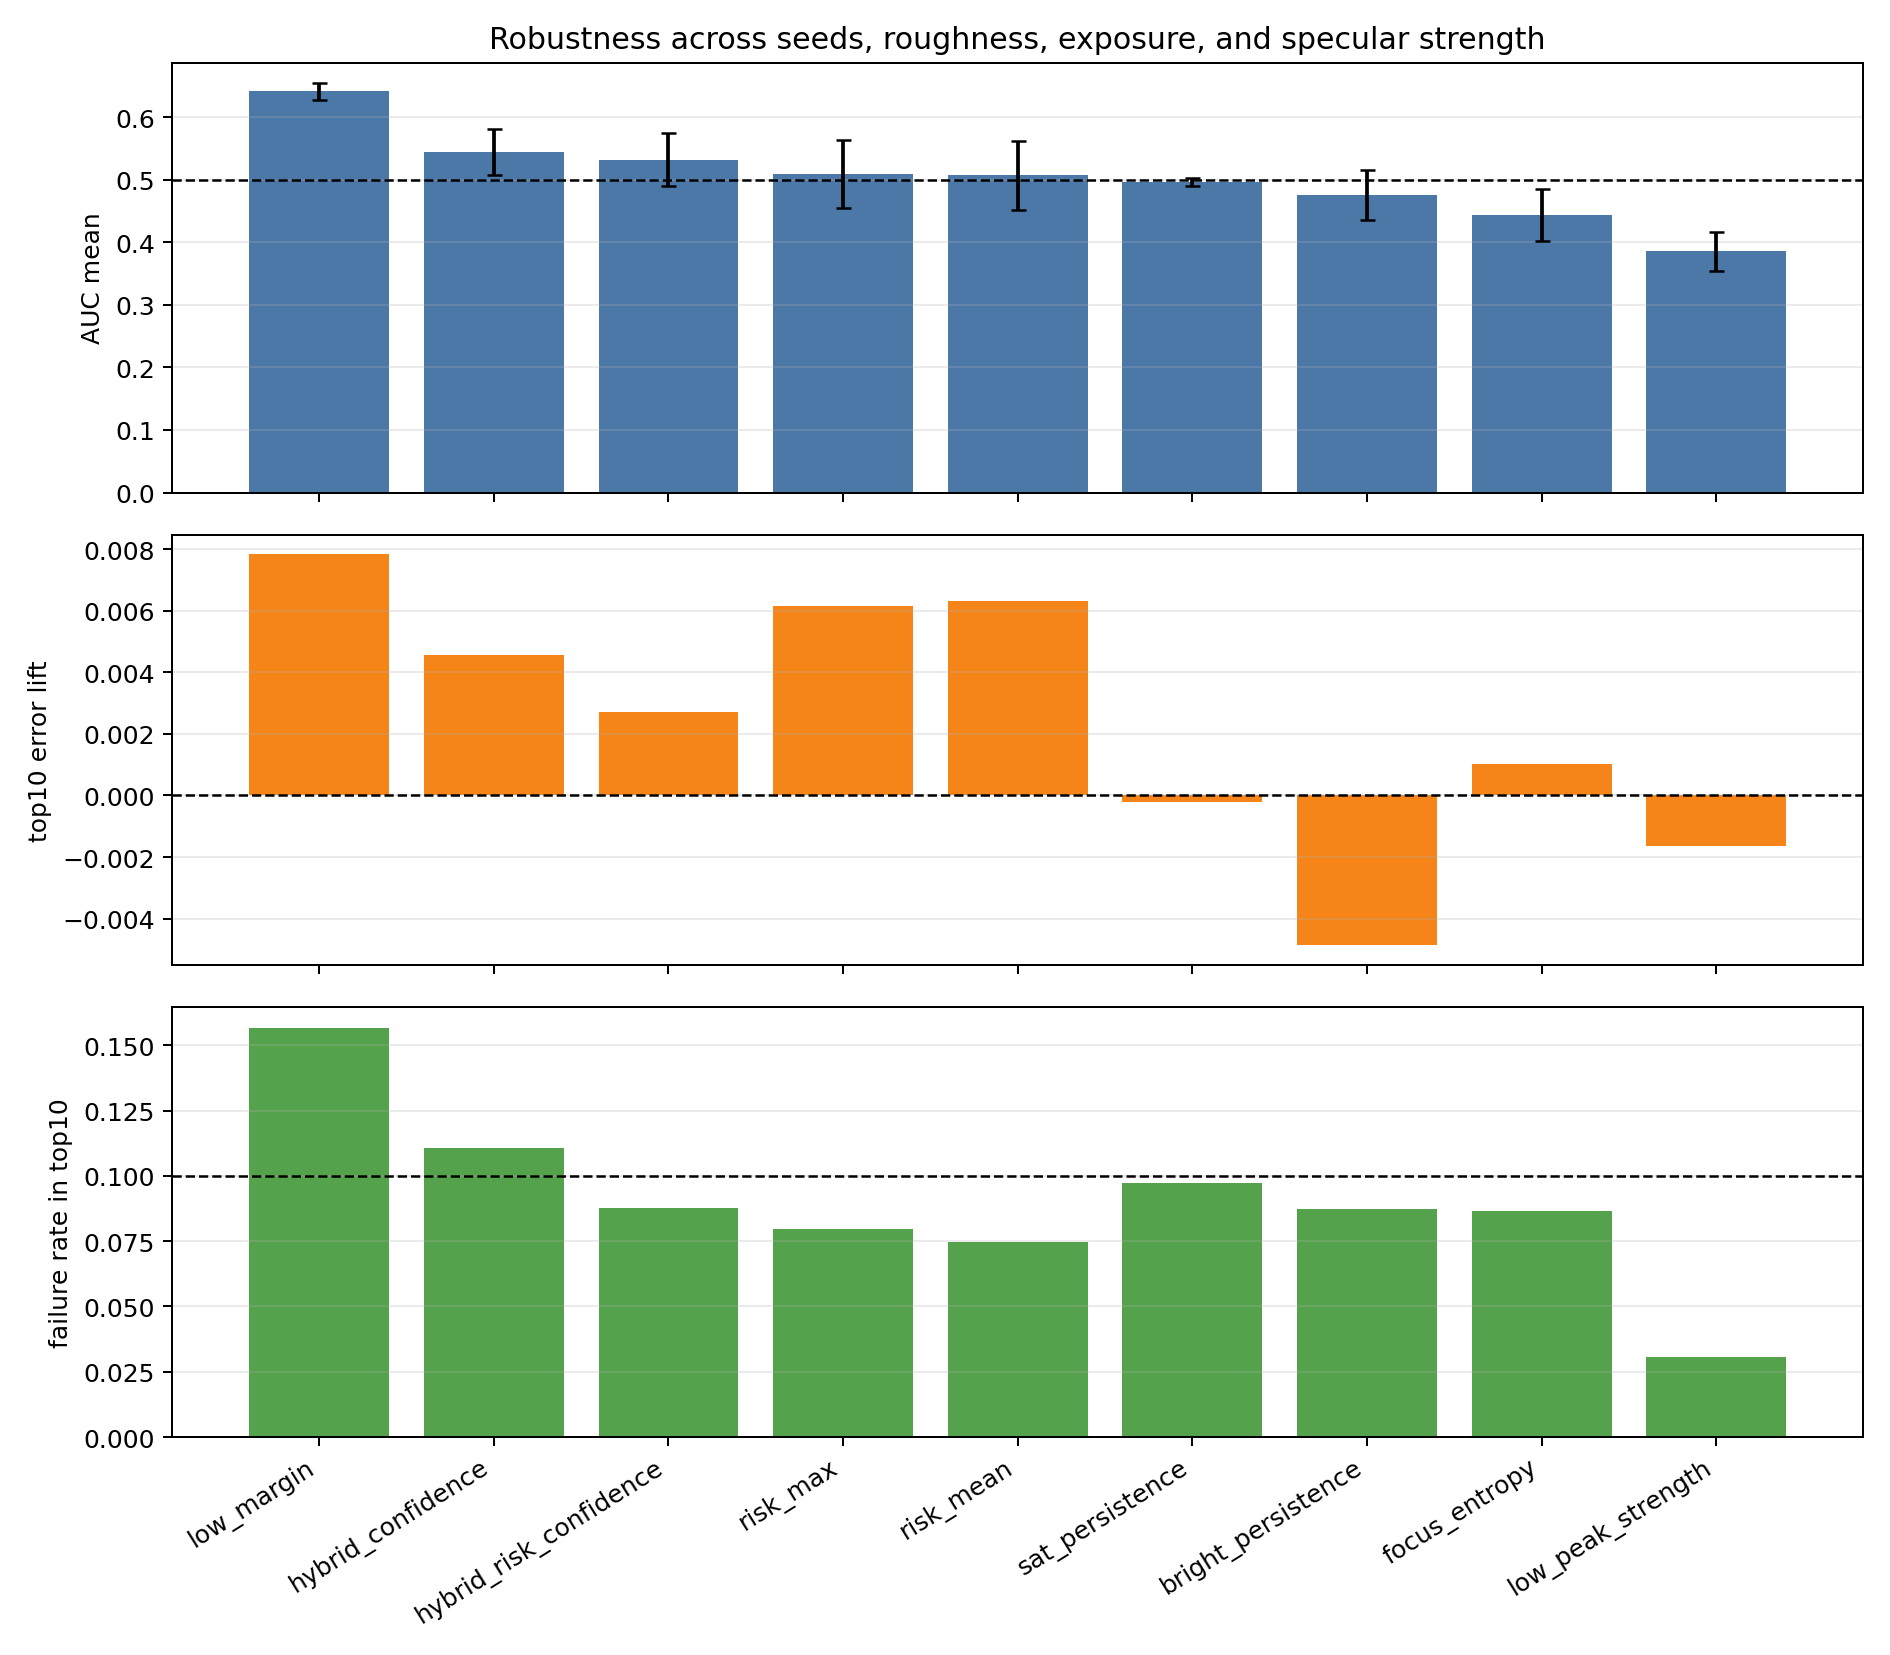
\includegraphics[width=\linewidth]{confidence_risk_robustness/confidence_risk_robustness_bars.png}
\caption{Mean AUC, top10 error lift, and failure rate for each diagnostic score.}
\end{figure}

\begin{figure}[htbp]
\centering
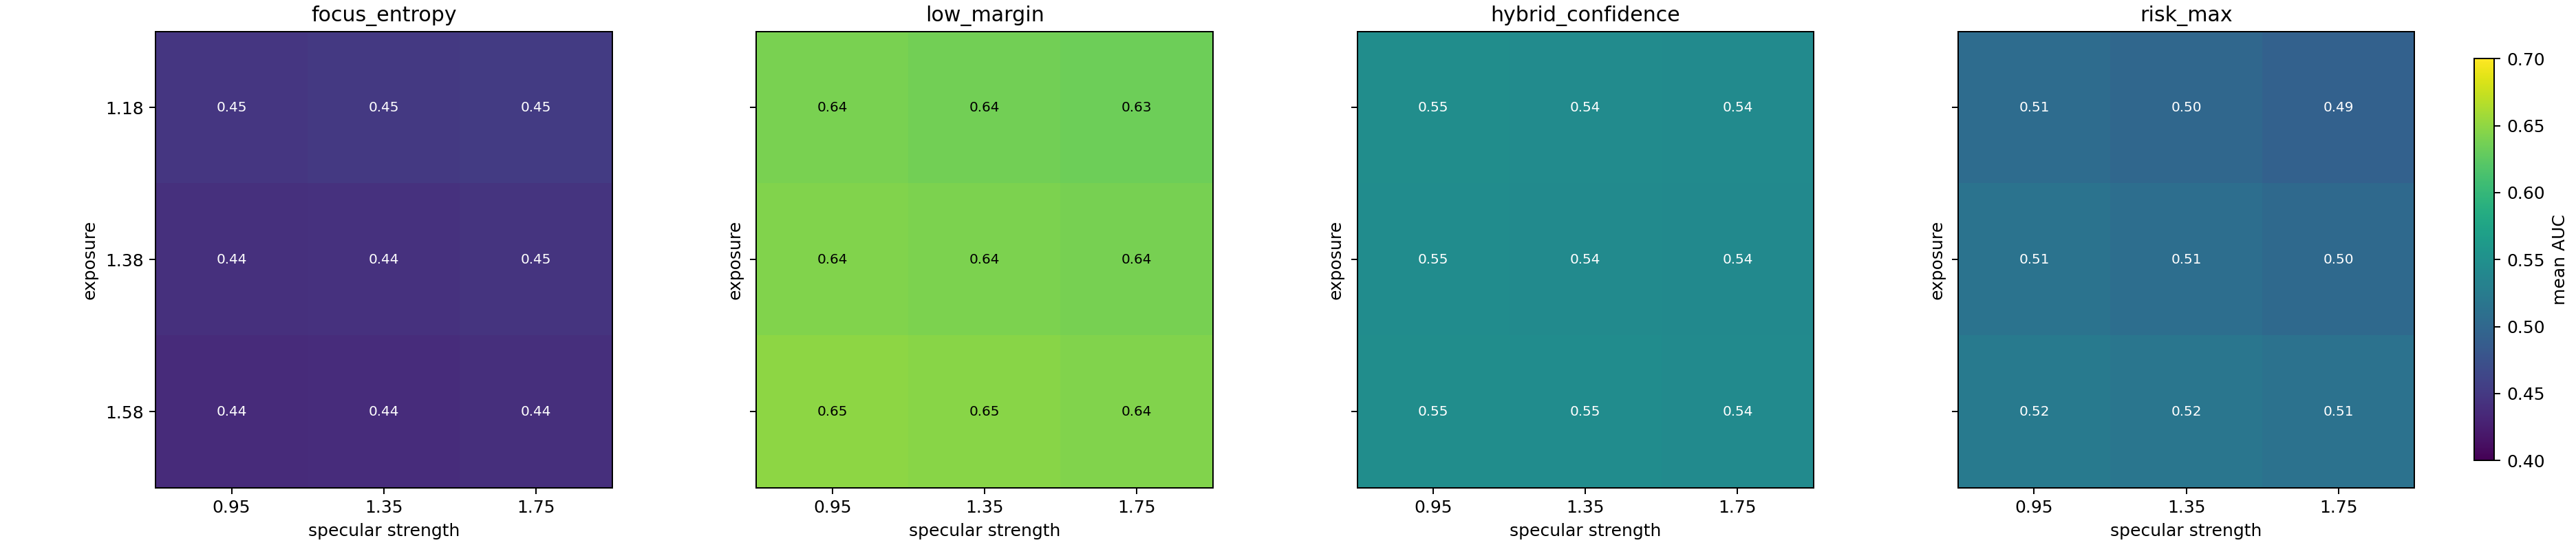
\includegraphics[width=\linewidth]{confidence_risk_robustness/confidence_risk_condition_heatmap.png}
\caption{Mean AUC across exposure and specular-strength settings.}
\end{figure}

\section{Key Findings}

\texttt{low\_margin} is the most stable DFF failure diagnostic in this sweep. Its mean AUC is 0.6412 with a standard deviation of 0.0133, and it remains above 0.55 in all tested conditions. Its top10 score region has an average failure rate of 15.68\%, clearly above the 10\% base rate. This result directly matches the DFF decision mechanism: when the top-1 and top-2 focus-response peaks are close, the argmax depth selection becomes sensitive to reflective pseudo-edges, weak texture, and local sampling perturbations.

The multi-condition result revises the previous single-case conclusion. Although \texttt{focus\_entropy} was the best score in one synthetic stack, it is not robust in the parameter sweep. Its mean AUC drops to 0.4438, with only 12\% of cases above random ranking. Entropy should therefore be treated as a candidate focus-curve ambiguity descriptor, not as the primary confidence prior.

Geometric glare-risk scores are close to random ranking: \texttt{risk\_mean} and \texttt{risk\_max} have mean AUCs of 0.5075 and 0.5087. This supports the interpretation that glare risk explains where reflective artifacts may originate, while DFF failure is more directly indicated by focus-response ambiguity.

\section{Method Revision}

The quality prior should be revised from a glare-dominated failure score to a focus-margin-dominated confidence score:

\begin{equation}
Q_{\mathrm{fail}}(x) =
\alpha (1 - M_{\mathrm{focus}}(x))
+ \beta H_{\mathrm{focus}}(x)
+ \gamma P_{\mathrm{sat}}(x),
\end{equation}

where $M_{\mathrm{focus}}$ is the top-2 focus margin, $H_{\mathrm{focus}}$ is focus entropy, and $P_{\mathrm{sat}}$ is saturation persistence. Based on the current sweep, $(1-M_{\mathrm{focus}})$ should be the main term, while entropy and saturation persistence should be auxiliary terms. Geometric glare risk should be used for physical interpretation, region-wise analysis, and optional gating rather than as a direct failure mask.

The weighted loss can be written as:

\begin{equation}
\mathcal{L} =
\mathrm{mean}\left((1 + \lambda Q_{\mathrm{fail}}) \cdot
\left|H_{\mathrm{pred}} - H_{\mathrm{gt}}\right|\right).
\end{equation}

\section{Paper-Ready Statement}

To examine the robustness of the proposed quality prior, we evaluate multiple no-reference diagnostic maps over 135 synthetic conditions with different random surfaces, roughness levels, exposure values, and specular strengths. The top-2 focus margin is the most stable indicator of DFF failure regions: the low-margin score achieves a mean AUC of 0.6412 with a standard deviation of 0.0133, and remains above 0.55 in all tested conditions. In contrast, geometric glare-risk scores are close to random ranking, with a mean AUC of approximately 0.51, while focus entropy is not robust across the parameter sweep. These results suggest that DFF failures are more directly associated with competition among focus-response peaks than with glare-prone geometry alone. We therefore use focus-margin confidence as the primary signal for loss weighting and no-reference quality diagnosis, while retaining glare risk as a physical prior for interpretation and region-wise analysis.

\section{Limitations}

The current sweep is still based on synthetic focal stacks, and the surface generator and exposure model are mechanism probes rather than calibrated microscope simulations. The conclusion should therefore be stated carefully: within the current simulator family, top-2 focus margin is more stable than entropy and glare risk as a DFF failure indicator. The next step is to verify whether low-margin regions align with visible DFF spikes, pseudo-edges, and unstable depth estimates in real ROIs.

\end{document}
